\documentclass[12pt]{article}

%%%Package Manager%%%
\setlength{\parindent}{4em}

\usepackage{amsmath}
\usepackage{setspace}
\usepackage{fancyvrb}
\usepackage{graphicx}
\usepackage{geometry}
\usepackage{hyperref}

\geometry{letterpaper, portrait, margin=1in}
%%%%%%%%%%

%%%Title Page%%%
\title{
	\begin{center}
		
\includegraphics[scale=0.5]{uga.png}\\
 	\end{center}
 	CSEE 4630\_3 Bioinstrumentation
\bigbreak Lab 1 - DIY Portable ECG (Heart Lab)
}

\author{
{\normalsize
\begin{tabular}{l c c}
& \textbf{Zachary Davis} & \\
& 811960668 & \\
\textbf{Category} & Zachdav@uga.edu & \\
\hline
Task A: Setup the Electrocardiogram Device & 5\% & \\
Task B: ECG Digital Signal Processing & 4\% & \\
Task C: Computing the Limb Leads \& Augmented Leads & 5\% & \\
Task D: Extraction of R Wave \& Vectorcardiogram Conversion & 6\% & \\
Task E: Stress Test Validation & 1.6\% & \\
\hline
\end{tabular}
}
}

\date{\bigskip
\today}
%%%%%%%%%%

%%%Content%%%
\begin{document}
	\maketitle
	\newpage
	
	\tableofcontents
	\newpage

	\section{Task A: Setup the Electrocardiogram Device}
		\subsection{Assembling the Provided Kit}
			\paragraph{}
				This year we were told that we were not going to solder the ECG because of 
				difficulties in previous years so we just used some male to female wires to 
				connect the ECG device the the oscilloscope and later the Arduino.  Once I 
				had the ECG device I used the arduino to power it, stuck the three leads to my
				chest and, connected the output to the oscilloscope just to varify that the device 
				was producing a signal.  The photo and data from the oscillosope is included in the 
				next section as it was more relavent to that section.
				
			\begin{center}
				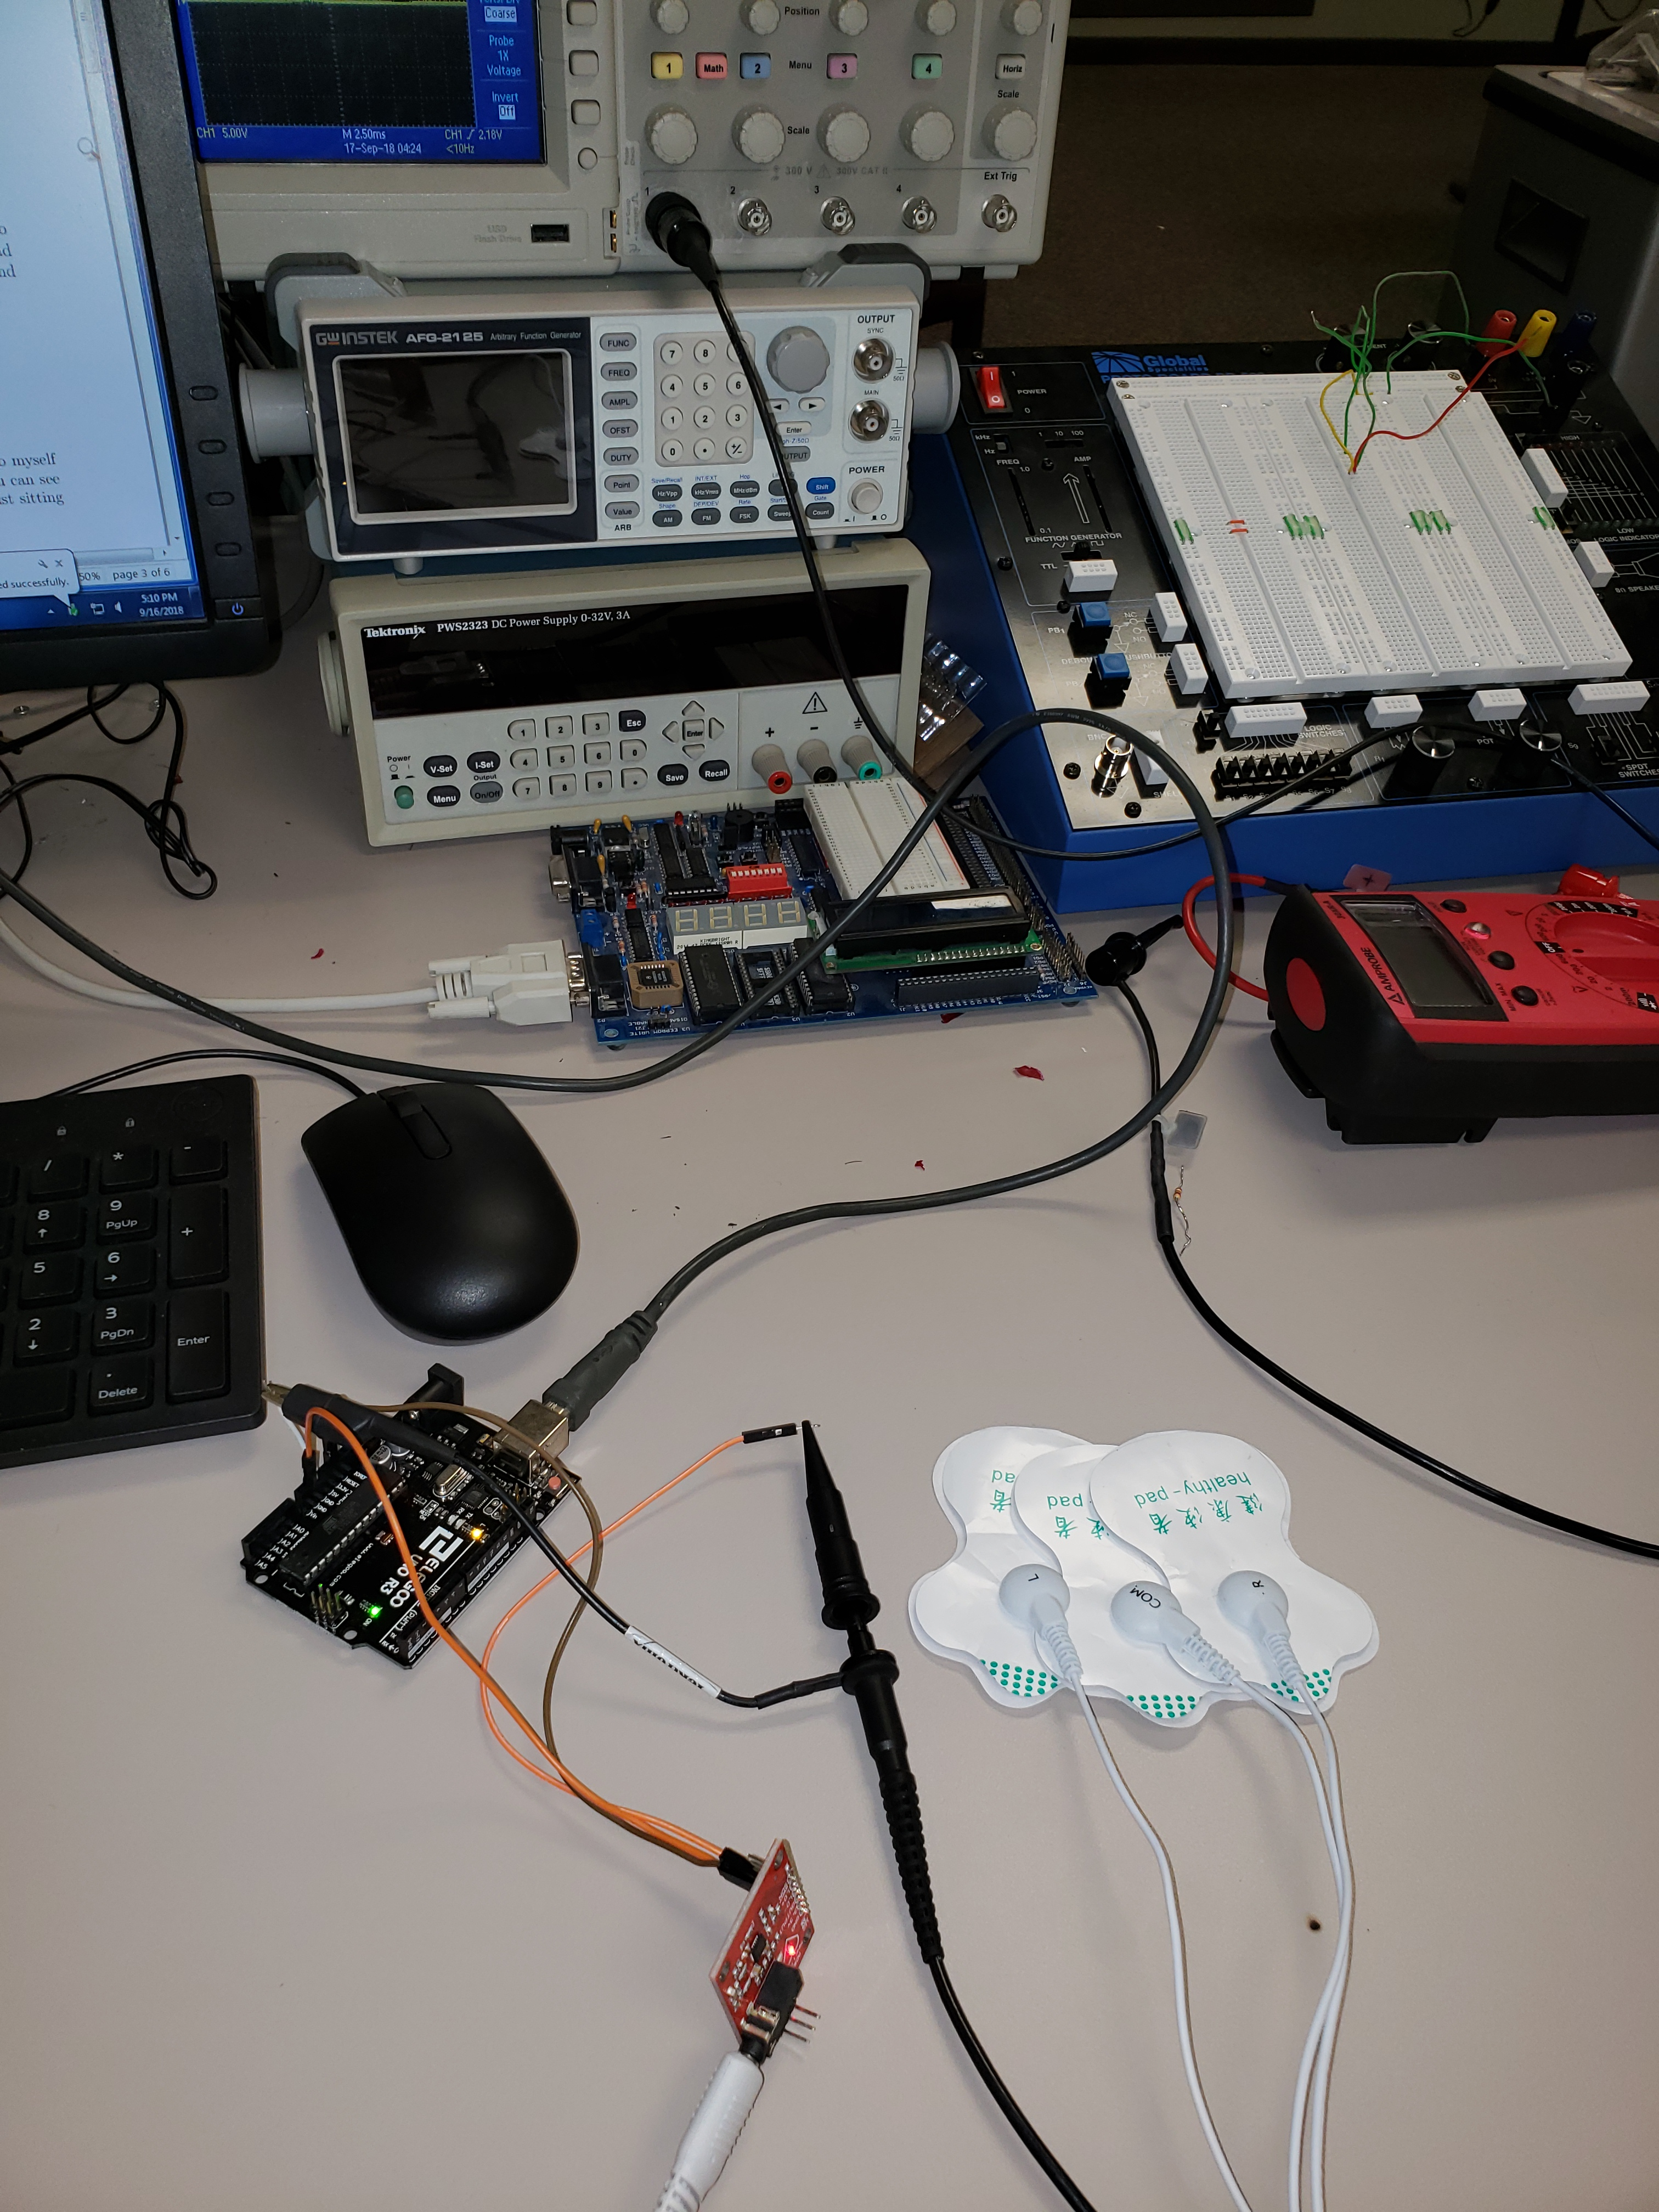
\includegraphics[scale=0.06]{part1.jpg}\\
			\end{center}
		
		\subsection{Obtaining From the ECG}
			\paragraph{}
				The following data was collected from the oscilloscope and the data points were saved
				 to a flash drive.  The oscilloscope was connected to the output of the ECG device which
				 had its three leads connected to me. I took the data points from the oscilloscope into 
				 excel and plotted them the show the data.
				 
			\begin{center}
				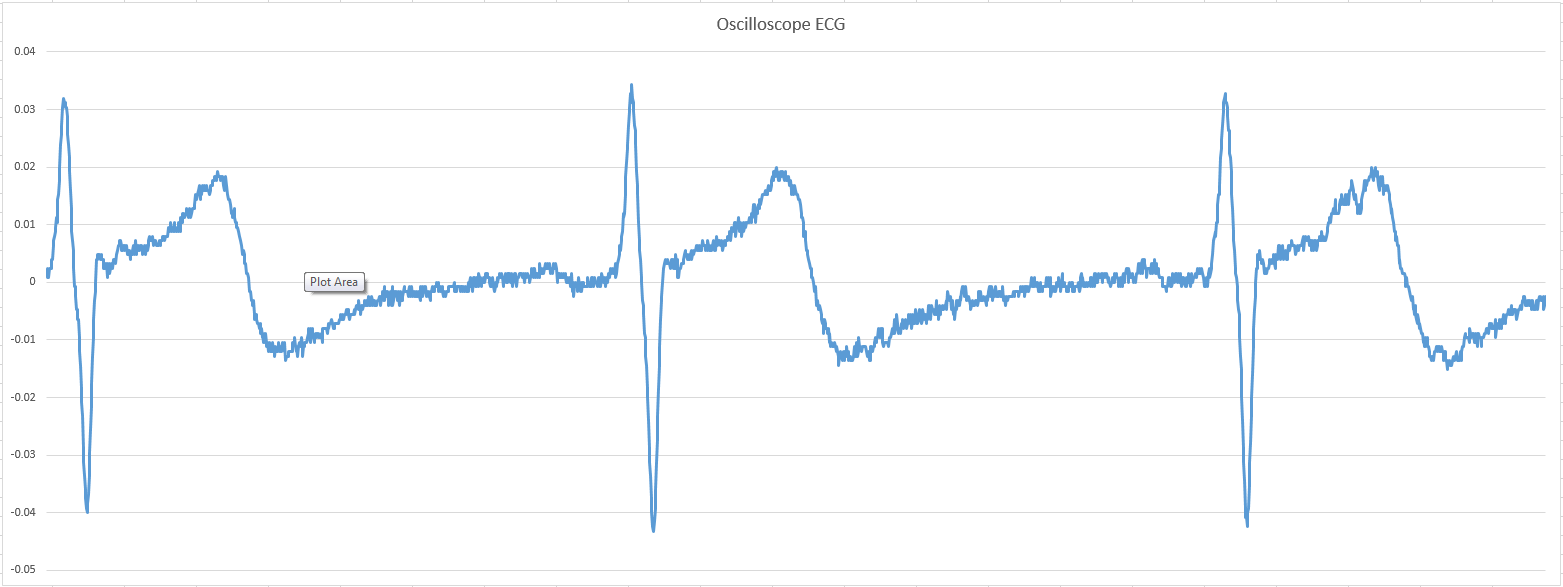
\includegraphics[scale=0.3]{oscope.png}\\
			\end{center}
	
	\section{Task B: ECG Digital Signal Processing}
		\subsection{Connecting the ECG to the Oscilloscope}
			\paragraph{}
				As I had done in the previous section I connected the ECG device input leads to myself 
				and 3V and ground to the arduino and finally the output to the oscilloscope as you can 
				see in the above picture.  The following picture is the signal I could see while i was just
				 sitting in a chair.		
				 
			\begin{center}
				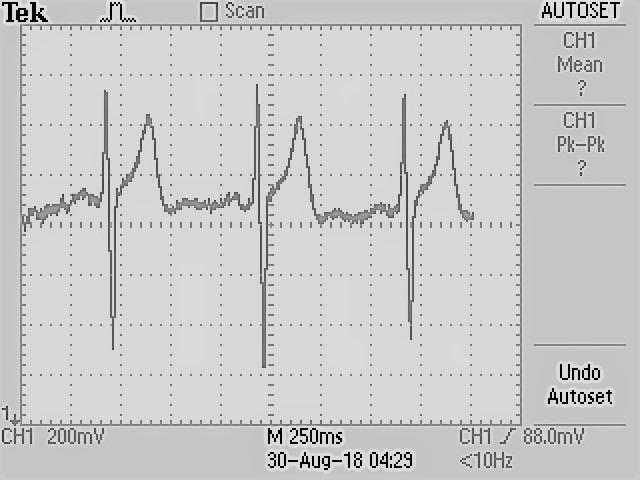
\includegraphics[scale=1]{o_1.jpg}\\
			\end{center}
		
		\subsection{Connect the ECG to the Arduino for Real-Time ECG Display}
			\paragraph{}
				Now that I have seen the ECG working the only thing that I changed in the setup was 
				connecting the ECG devices output pin to the A0 pin on the Arduino.  Then I was provided 
				an Arduino program that I cleaned up a little so I could better understand what was happening.
				The program reads in the output sensor value from A0 pin and prints that value with a 2 ms
				delay.\\
				
				\begin{center}
					\begin{verbatim}
						///Electrocardiogram Device///
						//Connect to A0//

						//Defining Constants and Variables
						const int analogInPin0 = A0;  
						int sensorValue0 = 0;        

						void setup() {
							// initialize serial communications at 9600 bps:
							Serial.begin(9600);
							delay(500);
						}

						void loop() {
							// read the analog in values:
							sensorValue0 = analogRead(analogInPin0);
  
							// print the results to the Serial Monitor:
							//Serial.print("val ");
  
							Serial.println(sensorValue0);
  
							delay(2);
							//delay(350);
						}
					\end{verbatim}
				\end{center}
				
				I can use the Arduino IDE to print the sensor output values to the serial monitor and plot the output data
 				versus a time scale calculated using the baud rate of 9600 to see my real time ECG or use the serial plotter 
				the actually view that data pre-plotted by the IDE.  Both are shown below.
				
				\begin{center}
					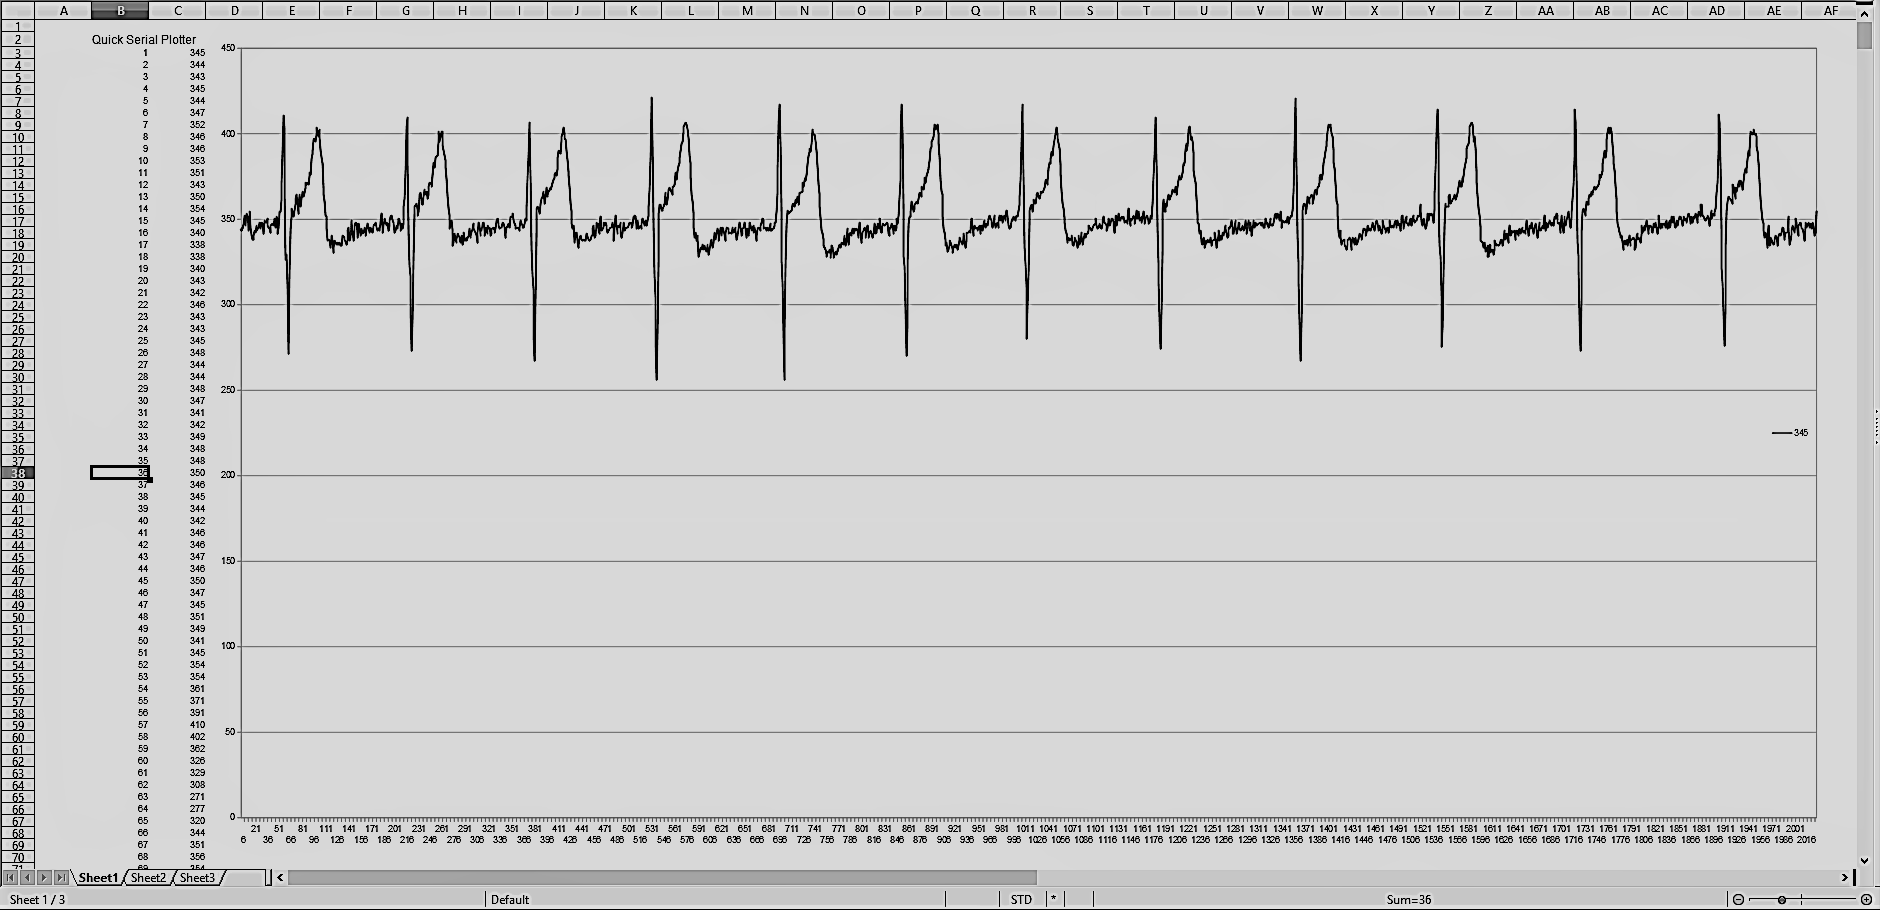
\includegraphics[scale=0.165]{monitor.PNG}\\
					\vspace{1cm}
					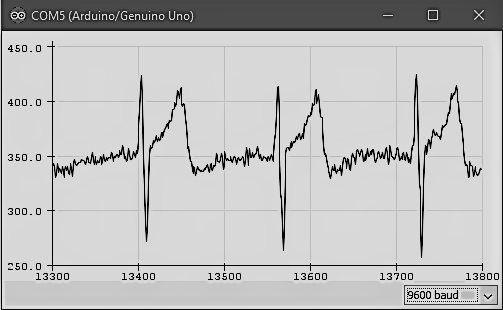
\includegraphics[scale=0.6]{plotter.PNG}
				\end{center}

				Now, in this task I am to take a 4 minute measurement of me increasing and decreasing my heart rate
				deliberately.  The instructions are to exercise for two minutes measuring at various intervals and then do 
				the same relaxing for two minutes.  For my experiement I will continually be taking my ECG while exercising
				for two minutes then relaxing for two minutes.  My `exercise' consists of leg lifts and holding my breath as
				not to increase the noise of the signal.  The resulting data was copied from the serial monitor and plotted
				using excel as before. The results are below.
				
		\subsection{Building A Band-Pass Filter for the ECG Signal}
			\paragraph{}
				For this task I needed to make a simple band pass filter the apply to the ECG to cutoff excessively low 
				and high frequencies from being plotted.  All I needed to determine is the high and low cutoff frequencies, 
				which i was able to find information on \href{https://link.springer.com/article/10.1007\%2Fs10527-016-9600-8}{here}. 
				 I then constructed the circuit below with a high pass cutoff frequency of 0.5 Hz and a low pass cutoff of 40 
				 Hz using a 3 Mohm\/0.1 uF and 40 Kohm\/0.1 uF respectively.  The results of the filter are shown below.

				\begin{center}
					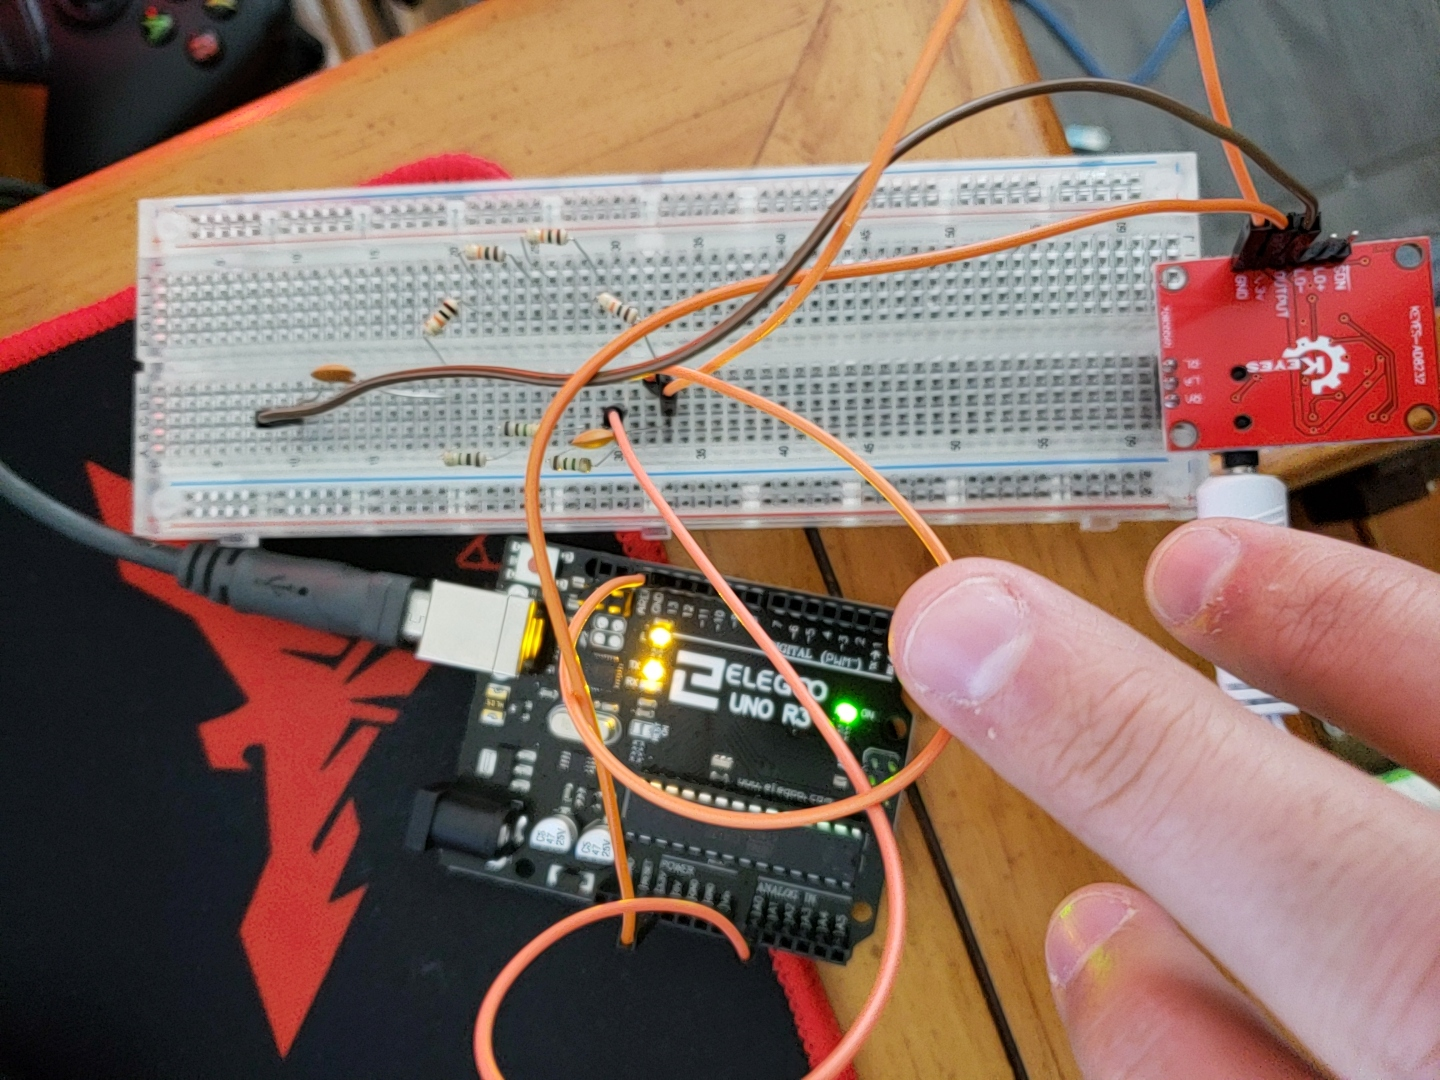
\includegraphics[scale=0.12]{filter.jpg}\\
					\vspace{1cm}
					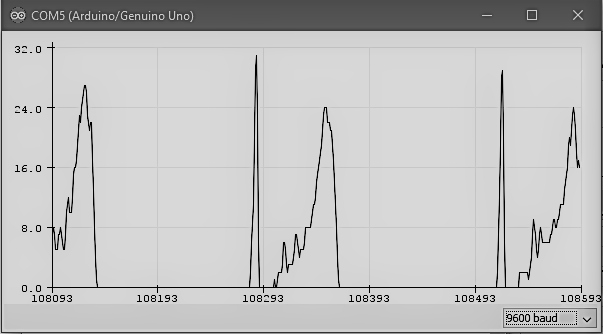
\includegraphics[scale=0.4]{filter_plotter.PNG}
				\end{center}

				While the signal does look cleaner than the previous ones shown even though I used a high pass filter with a cutoff of essentially
				zero the P, Q, T, and U wave are getting cutoff. If I had the time i would instead use matlab to apply a software solution as I could
				more actually choose the cutoff frequencies and have yet and even cleaner solution.
				
	\section{Task C: Computing the Limb Leads \& Augmented Leads}
		\subsection{Computing the Voltages for Lead I, II, and III}
			\paragraph{}
				For this part of the lab I needed to record the signal of lead I and lead II using the ECG device from the serial plotter simultaneously
				then i can subtract lead I from lead II the result being lead III. Finally I graphed all three leads to visualize and verify the data for 
				comparison in excel which you can see below. It is worth mentioning that I needed to measure the voltages at both leads simultaneously
				to be able to calculate an accurate lead three, which means i was using multiple alligator clips on the pads making the signal slightly more
				noisy.

				\begin{equation}
					L_{III} = L_{II} - L_I
				\end{equation}

				\begin{center}
					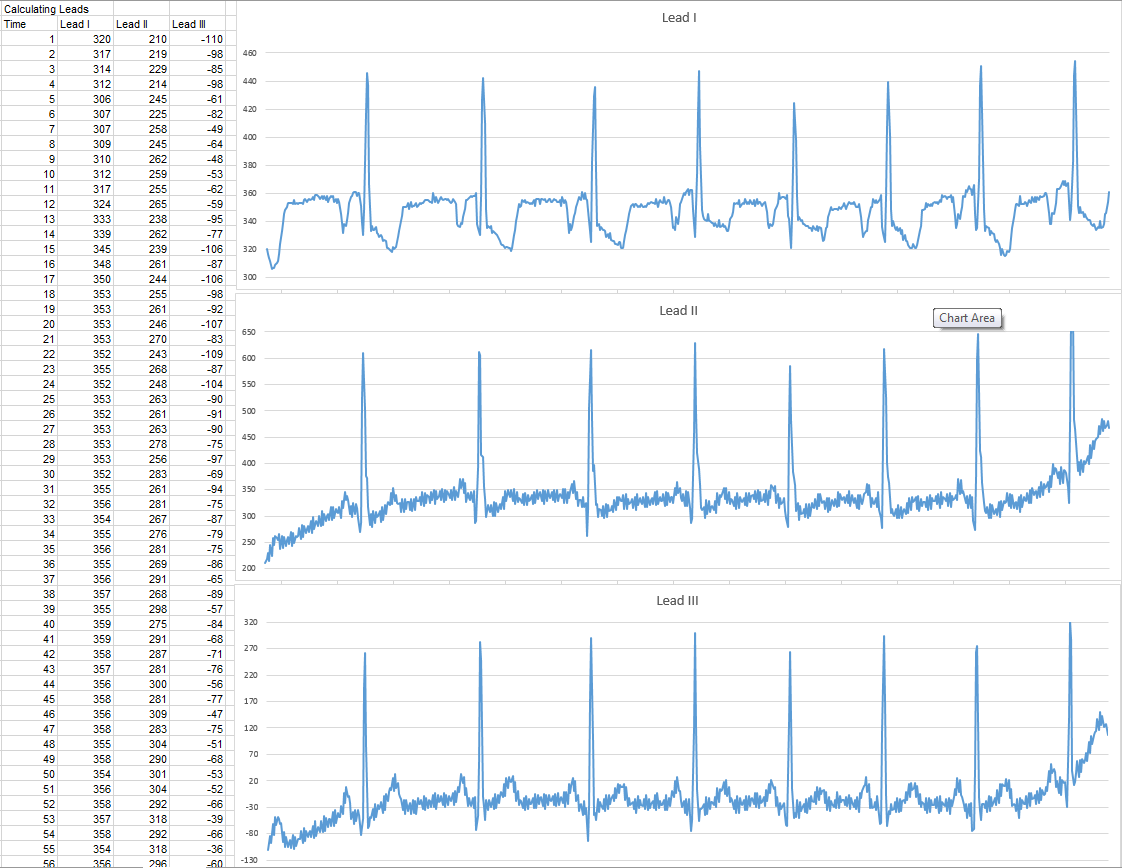
\includegraphics[scale=0.28]{3leads.PNG}\\
				\end{center}

				This is how the arduino source code had to be changed to allow for two analong inputs simultaneously.  The two values are printed on one
				output line seperated by a comma so they can easily be compied and formatted into excel to be graphed.

				\begin{center}
					\begin{verbatim}
						///Electrocardiogram Device///
						//Connect to A0//

						//Defining Constants and Variables
						const int analogInPin0 = A0;  
						int sensorValue0 = 0;

						const int analogInPin0 = A1;
						int sensorValue1 = 0;

						void setup() {
  							// initialize serial communications at 9600 bps:
 							Serial.begin(9600);
 							delay(500);
						}

						void loop() {
 				 			// read the analog in values:
 							sensorValue0 = analogRead(analogInPin0);
  							sensorValue1 = analogRead(analogInPin1);
  
  							// print the results to the Serial Monitor:
  							//Serial.print("val ");
  
 							Serial.print(sensorValue0);
  							Serial.print(",");
  							Serial.println(sensorValue1);
  
 	 						delay(2);
  							//delay(350);
						}
					\end{verbatim}
				\end{center}

		\subsection{Calculating aVL, aVR, and aVF}
			\paragraph{}
				Now that we have the values of leads I, II, and III we can use three equations from Wilson's augmented leads to calculate the three 
				augmented leads, which are shown here.

				\begin{equation}
					aV_L = \frac{2V_L-V_R-V_F}{3}
				\end{equation}
				\begin{equation}
					aV_R = \frac{2V_R-V_L-V_F}{3}
				\end{equation}
				\begin{equation}
					aV_F = \frac{2V_F-V_R-V_L}{3}
				\end{equation}

				If I re-group the terms in terms of leads I, II, and III i can use the data i collected in the previous section to calculate all the augmented leads 
				very easily.

				\begin{equation}
					aV_L = \frac{V_1-V_3}{3}
				\end{equation}
				\begin{equation}
					aV_R = \frac{-V_1-V_2}{3}
				\end{equation}
				\begin{equation}
					aV_F = \frac{V_2+V_3}{3}
				\end{equation}

				Now you can see the three graphs of each of the augmented leads that i calculated from the data i collected from lead I and lead II.

				\begin{center}
					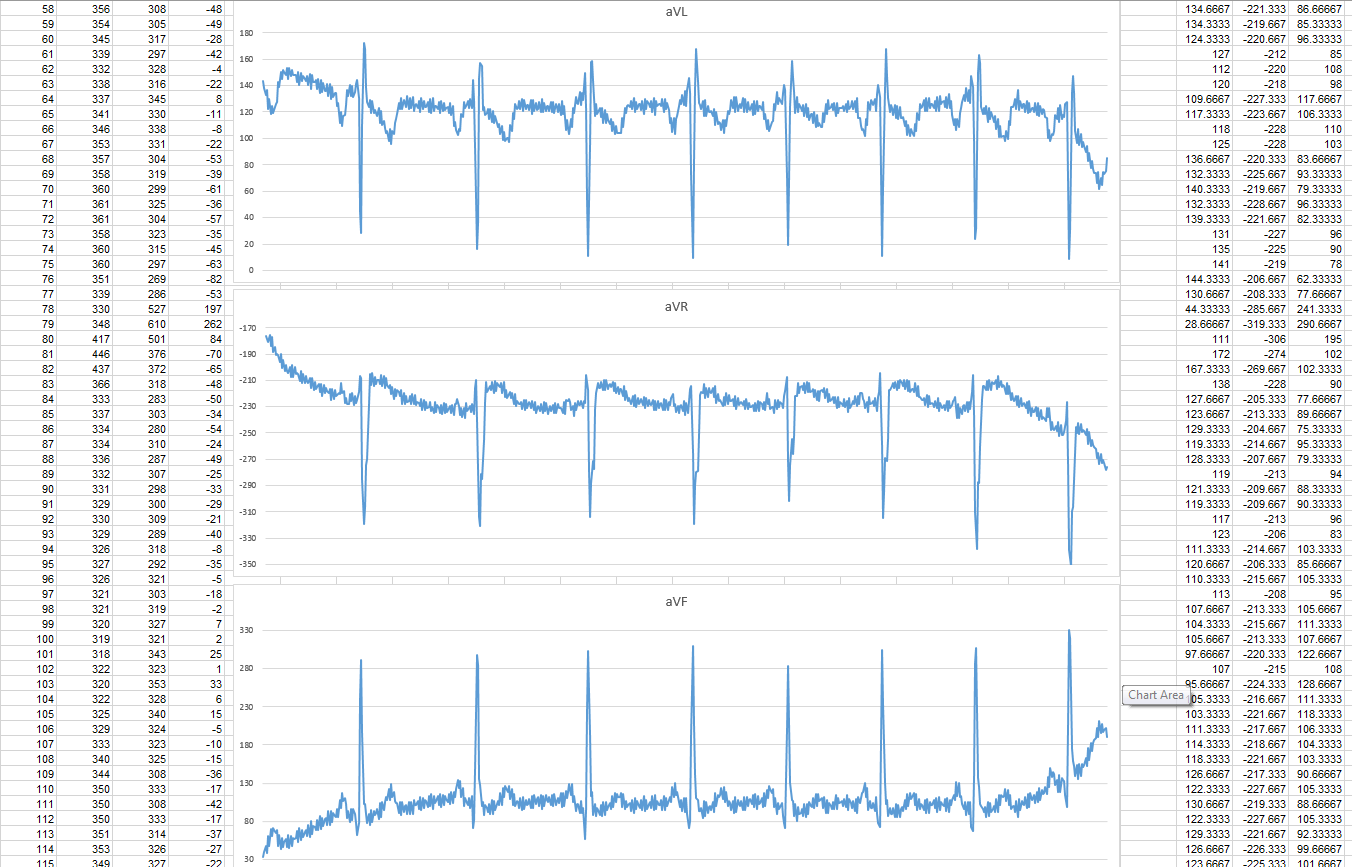
\includegraphics[scale=0.28]{augmented.PNG}\\
				\end{center}

		\subsection{Computing a Vectorcardiogram in the Frontal Plane}
			\paragraph{}
				For this section I need compute the three values of the vectorcardiogram. Now we can not reasonably collected data for the other 6 
				leads needed in a 12 lead ECG that will lets perfectly convert to a VCG but we do have lead I and II so we can convert to a VCG in the 
				frontal plane.  To do this we need to multiply the matrix of lead I and II with the matrix of dower coefficents that correlate to leads I and
				II. This will give us the values of X, Y and, Z, which I can then graph to show the VCG strictly in the frontal plane. 

				\begin{center}
					$\begin{pmatrix}
						X \\
						Y \\
						Z
					\end{pmatrix}
					=
					\begin{pmatrix}
						I \\
						II
					\end{pmatrix}
					*
					\begin{pmatrix}
						0.156 & -0.009 \\
						-0.227 & 0.886 \\
						0.021 & 0.102
					\end{pmatrix}$
				\end{center}

				\begin{center}
					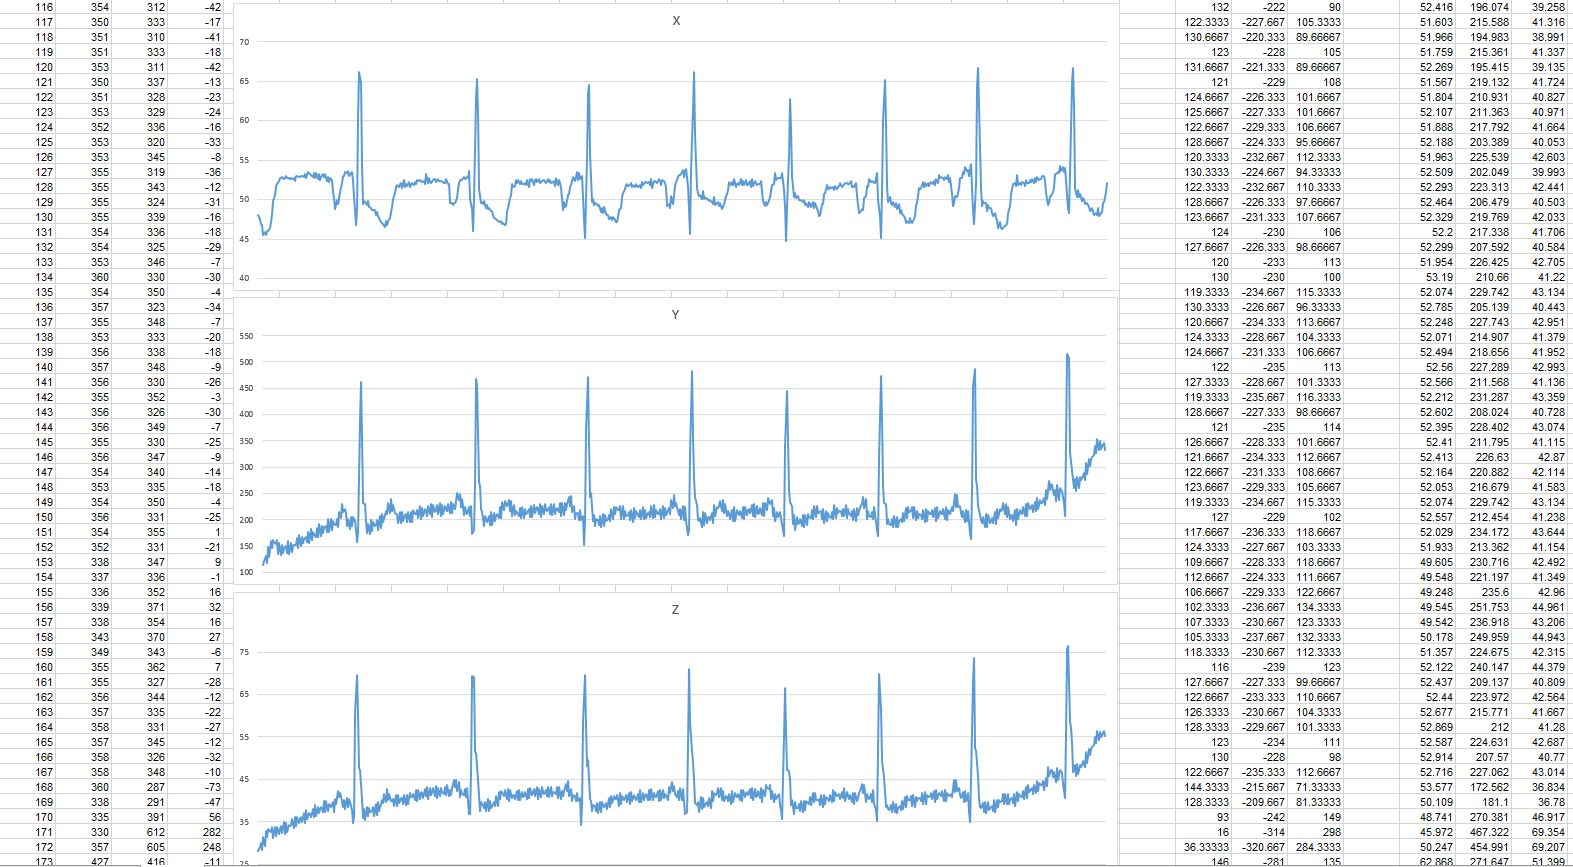
\includegraphics[scale=0.3]{vector.PNG}\\
				\end{center}

				It would appear that my conversion to a VCG is successful since X, Y, and, Z correlate with Lead I, II, and III respectively except for, of 
				course the amplitude.  In our case we only used two leads and some math to get to this point but with a VCG in the frontal plant we only
				need 2 leads rather than all three.

	\section{Task D: Extraction of R Wave \& Vectorcardiogram Conversion}
		\paragraph{}
			The purpose of this task is to learn and understand making an heart rate variability plot and practice measuring the R to R intervals on an ECG plot. To 
			complete this i took the plot from section 2.2 and created a corresponding HRV plot.  There are many ways to tackle this issue the most effective would
			be to have lines of code that save and print a max in a certain threshold but to create a plot once you already have the serial output data you could use 
			matlab or other various programs but, I found that the easiest way was to use a vary simple excel function.  Below is my resulting HRV and it seems to match
			the ECG plot and is relatively constant which is good as well.

			\begin{center}
				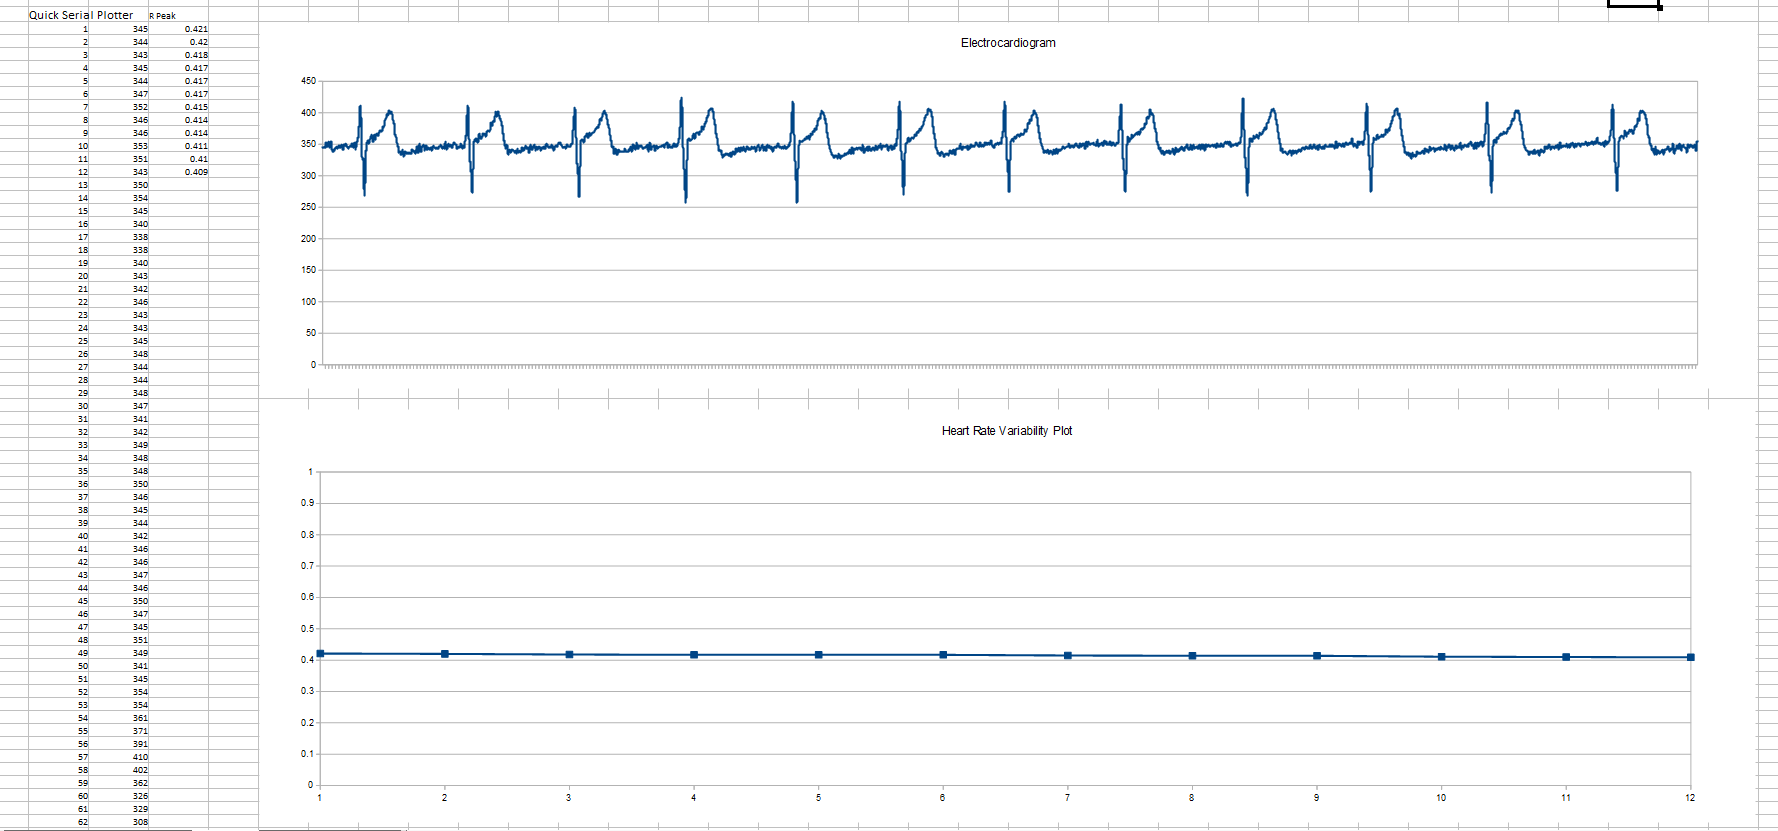
\includegraphics[scale=0.3]{hrv.PNG}\\
			\end{center}

	\section{Task E: Stress Test Validation}
		\paragraph{}
			In the final section the goal is to exercise for three minutes then rest for three minutes then finally exercise for three more minutes and take 
			measurement every minute on the oscilloscope.  After i completed this i took all the data and complied it in excel and created a graph that shows
			each of the ten measurements stacked on top of each other and a legend of course.  This was an interesting way to look at the data because you 
			could compare the heart rates at the different times pretty directly, but admittedly with ten different measurements it can be pretty hard to read.
			That is why after that i created a heart rate variability graph to get an easier to see more full picture in the change in my heart rate.

			\begin{center}
				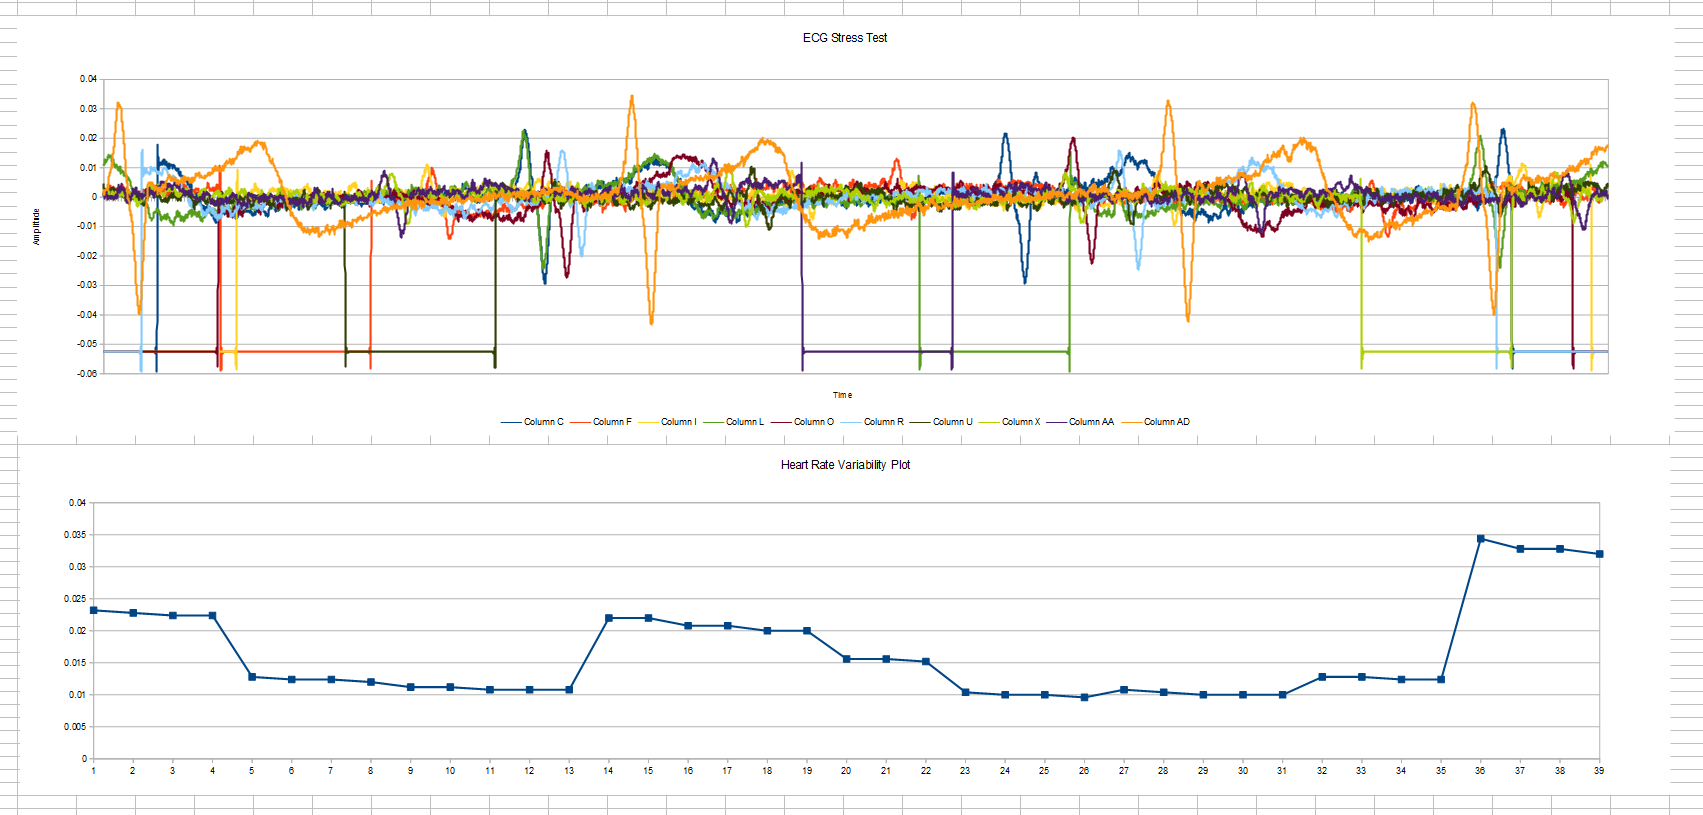
\includegraphics[scale=0.35]{stress.PNG}\\
			\end{center}
\end{document}
%%%%%%%%%%